\documentclass{article}

% if you need to pass options to natbib, use, e.g.:
% \PassOptionsToPackage{numbers, compress}{natbib}
% before loading nips_2016
%
% to avoid loading the natbib package, add option nonatbib:
% \usepackage[nonatbib]{nips_2016}

\usepackage{nips_2016}

% to compile a camera-ready version, add the [final] option, e.g.:
% \usepackage[final]{nips_2016}

\usepackage[utf8]{inputenc} % allow utf-8 input
\usepackage[T1]{fontenc}    % use 8-bit T1 fonts
\usepackage{hyperref}       % hyperlinks
\usepackage{url}            % simple URL typesetting
\usepackage{booktabs}       % professional-quality tables
\usepackage{amsfonts}       % blackboard math symbols
\usepackage{nicefrac}       % compact symbols for 1/2, etc.
\usepackage{microtype}      % microtypography
\usepackage{amsmath}
\usepackage{listings}
\usepackage{graphicx}
\usepackage{textcomp}
\usepackage{graphicx}
\title{Using Neural Networks to Effectively Classify Hand-Written Digits of the MNIST Dataset}

% The \author macro works with any number of authors. There are two
% commands used to separate the names and addresses of multiple
% authors: \And and \AND.
%
% Using \And between authors leaves it to LaTeX to determine where to
% break the lines. Using \AND forces a line break at that point. So,
% if LaTeX puts 3 of 4 authors names on the first line, and the last
% on the second line, try using \AND instead of \And before the third
% author name.

\author{
  Chetan Gandotra\thanks{Use footnote for providing further
    information about author (webpage, alternative
    address)---\emph{not} for acknowledging funding agencies.} \\
  Department of Computer Science\\
  UC San Diego\\
  San Diego, CA 92093 \\
  \texttt{cgandotr@ucsd.edu} \\
}

\author{
  David S.~Hippocampus\thanks{Use footnote for providing further
    information about author (webpage, alternative
    address)---\emph{not} for acknowledging funding agencies.} \\
  Department of Computer Science\\
  Cranberry-Lemon University\\
  Pittsburgh, PA 15213 \\
  \texttt{hippo@cs.cranberry-lemon.edu} \\
  %% examples of more authors
  %% \And
  Chetan Gandotra \\
  UC San Diego \\
  9500 Gilman Drive \\
  \texttt{cgandotr@ucsd.edu} \\
  %% \AND
  %% Coauthor \\
  %% Affiliation \\
  %% Address \\
  %% \texttt{email} \\
  %% \And
  %% Coauthor \\
  %% Affiliation \\
  %% Address \\
  %% \texttt{email} \\
  %% \And
  %% Coauthor \\
  %% Affiliation \\
  %% Address \\
  %% \texttt{email} \\
}
\newcommand\thicktilde{{\lower.74ex\hbox{\texttt{\char`\~}}}}
\begin{document}
% \nipsfinalcopy is no longer used

\maketitle

\begin{abstract}
This report discusses the second programming assignment of our course CSE 253: Neural Networks and Pattern Recognition, its solutions and the inferences we drew. A variable layer neural network was implemented from the scratch and observations were made based on various parameters and before/after adding certain trades of tricks as discussed in Yann LeCun's famous paper "Efficient BackProp". The data-set used was the famous MNIST data-set and a ten-way classification was performed on it. A test data-set accuracy in excess of 97\% was achieved using various mechanisms and tricks, which is almost at par with the accuracy reported by LeCun on his website.
\end{abstract}

\section{Task 3: Implementing Neural Network and Gradient Calculation}
\subsection{Introduction}
This problem asks us to build a neural network from scratch using our derivations from Problem 2. We are required to read the MNIST data-set and normalize the data by dividing each pixel value by 255, followed by subtracting the mean over all of the pixels in each image. We have been asked to use the softmax activation function for output layer and logistic activation function for hidden layers. We need to check our code for gradient computation by using the following numerical approximation formula for each weight:
\begin{align}
\frac{d}{dw}E^n(w) \approx \frac{E^n(w+\epsilon) - E^n(w-\epsilon)}{2\epsilon}
\end{align}
Finally, using the update rule from 2(c), we will perform gradient descent and report our accuracy on training and test data-sets.
\subsection{Methodology}
The MNIST data-set was downloaded and extracted into local variables using existing libraries available online on GitHub. [Note that we used the same off-the-shelf GitHub library for PA1 as well]. Once we had the data, we normalized it using the instructions mentioned. Each value was divided by 255, and the row-wise mean was subtracted from each element in that row.

Then, a neural network was implemented that included forward propagation, back-propagation and weight update steps. The activation functions used were logistic (for hidden layer) and softmax (for output layer). Thus, our neural network had three layers - one input layer of size 784, one hidden layer of size 300 and lastly, the output layer of size 10. The hidden layer was chosen to have 300 units as many of the experiments on LeCun's website had 300 hidden units in them. Note that the output was converted into a "one-hot" representation form. The learning rate was set to be 0.0000044 (obtained using - 0.22/50k examples) after much experimentation and inferring the best learning rate. 

The full batch of 50k examples was given to the neural network to learn, and a stopping condition was enforced using a neural network. If at any point 5 or more continuous validation error (mis-classification error) values increased, we stopped training our model and exited. All the previous weights were stored and the weights having least error on validation set were selected to be the optimal weights. Note that we also used cross entropy error on validation set to enforce a stopping condition and it yielded a similar learning pattern. Due to this, we decided to go with either one of the two error calculations.

To sum:
$\eta$ = 0.0000044, examples = 50,000 (full batch used), convergence criteria = Validation set mis-classification error 

For 3(d), we computed the slope with respect to one weight using the numerical approximation in equation (29). The value of $\epsilon$ was taken to be 0.01 and the gradient for weights of each layer was compared to our gradient calculation method. Both the gradients were calculated and stored in lists and then subtracted. Finally, the subtracted result was used to draw inferences.

\subsection{Results}
The gradient difference findings are as under:

Maximum Absolute Difference in $W_{ij}$: 5.01416981156e-07

Maximum Absolute Difference in $W_{jk}$: 0.000900066795115

Mean Difference for $W_{ij}$: 3.80757313778e-08

Mean Difference for $W_{jk}$: 9.02485484117e-05

The detailed differences for every weight in $W_{ij}$ and $W_{jk}$ are given in attached files - GradientDifferenceIJ.csv and GradientDifferenceJK.csv, respectively.

Using gradient descent on full training set (minus the validation set) resulted in an accuracy of 91.8\% on the training set and 91.7\% on the test-set in 527 iterations. Note that validation error was used as a means of stopping criteria. 
\begin{figure}[h!]
  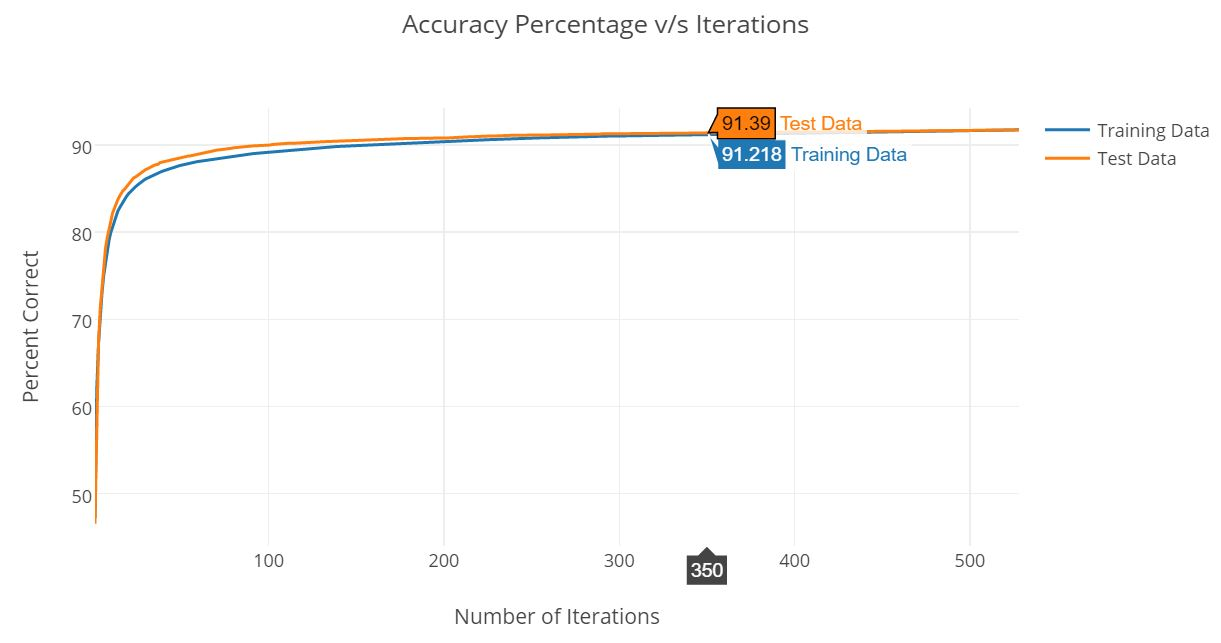
\includegraphics[width=120mm]{graphs/Q3e_Pt22_fullBatch_500iter_new.JPG}
  \caption{Accuracy Percentage v/s Iterations for Full Batch in 2-layer Neural Network with 300 Hidden Units} 
  \label{fig:3e}
\end{figure}

Graph \ref{fig:3e} shows the percent correct plots for training and test data over 500+ iterations. As shown in the graph, at 350th iteration, we had a training accuracy of 91.39\% and test accuracy of 91.218\%.

\subsection{Discussion}
The gradient calculation from part 3(d) performed as expected. With an $\epsilon$ value 0.01, the difference of gradients agreed in O($\epsilon^2$), i.e., $10^{-4}$. This tells us that our gradient computation is reliable and can be relied upon for the purpose of this assignment. 

The results of 10-way classification using a two-layer neural network on MNIST data-set were satisfactory. The convergence slows down a lot as number of iterations increase and more than 500 iterations were required to achieve an accuracy of 91.7\% on the test set. As you can see in graph \ref{fig:3e}, there was little improvement on the training and test accuracies after 200 iterations and the graph was this point was almost a straight line parallel to the iteration axis. This gives us a motivation to use and try out the various tricks of trades mentioned by Yann LeCun et al in the famous paper "Efficient BackProp".
\newpage
\section{Task 4: Adding the "Tricks of the Trade"}

\subsection{Introduction}
In this section, we would apply certain tricks from a famous paper by Yann Lecun and analyze their effect on the performance of our neural network. Particularly, we would be doing following things:
\begin{enumerate}
  \item We would shuffle the data and apply stochastic gradient descent over a mini-batch of varying size to analyze the effect of mini-batch size on performance.
  \item We would use a different sigmoid function ($1.7159 \: tanh(\frac{2x}{3})$) as an activation function for the hidden layer and observe its effect.
  \item We would observe the effects when weights are initialized in a specific way suggested in the paper.
  \item We would add a momentum term in the update rules and would observe its effects.
\end{enumerate}

\subsection{Methodology}
We will be applying all the above task incrementally and observe their effects. For the first part, we would randomly shuffle the data using numpy library's inbuilt shuffle function. Then we consider mini-batches of size 50, 128 and 500 and analyze their performance on our data. Learning rate is set to 0.1 and number of units in hidden layer is 300.

For the second part, we choose mini-batch size of 128 and use the sigmoid function ($1.7159\:tanh(\frac{2x}{3})$) as an activation function for the hidden layer. The value of the hyperparameters is same as that of previous part. Derivative of this function could be found as following.
\begin{align*}
\frac{d}{dx} 1.7159 \: tanh(\frac{2x}{3}) = 1.7159 \: (1 - tanh^{2}\left(\frac{2x}{3}\right)) \frac{2}{3} 
\end{align*}
\begin{align*}
= 1.1439 \: (1 - tanh^{2}\left(\frac{2x}{3}\right))
\end{align*}


For the next part, we initialize the weights by random samples drawn from normal distribution with $\mu=0$ and $\sigma = \sqrt[]{\frac{1}{fan-in}}$ where the $fan-in$ is the number of units in the respective layer. The value of the hyperparameters is same as that of previous part.

For the last part, we add a momentum term in our update rule. Now the update rules for the weights would look like following:

\begin{align*}
w_{jk}^{t+1} = w_{jk}^{t} - \eta \frac{\partial E}{\partial w_{jk}^{t+1}} + \beta(w_{jk}^{t} - w_{jk}^{t-1})
\end{align*}
\begin{align*}
w_{ij}^{t+1} = w_{ij}^{t} - \eta \frac{\partial E}{\partial w_{ij}^{t+1}} + \beta(w_{ij}^{t} - w_{ij}^{t-1})
\end{align*}

where $\beta$ controls how much weight the momentum term should have. For our experiments, we have considered the value of $\beta$ as 0.9. The value of other hyperparameters is same as that of previous part.

We'll run all the experiments on 1000 iterations with early stopping horizon value of 5. However, since our empirical results showed no significant improvement after 100 iterations, we will show the results only on first 100 iterations for our comparative study (otherwise the shape of curve would not be visible clearly). Another motivation for taking first 100 iterations for plotting is that any setting could lead to best possible value when allowed to run sufficiently large time, but that wouldn't give us a clear picture of effects of the tricks we are applying.



\subsection{Results}

Results for each of the part is shown below:

1 - Results for shuffling of data and applying stochastic gradient descent over a mini-batch of varying size are shown below.

\pagebreak
\begin{figure}[h!]
  \centering
  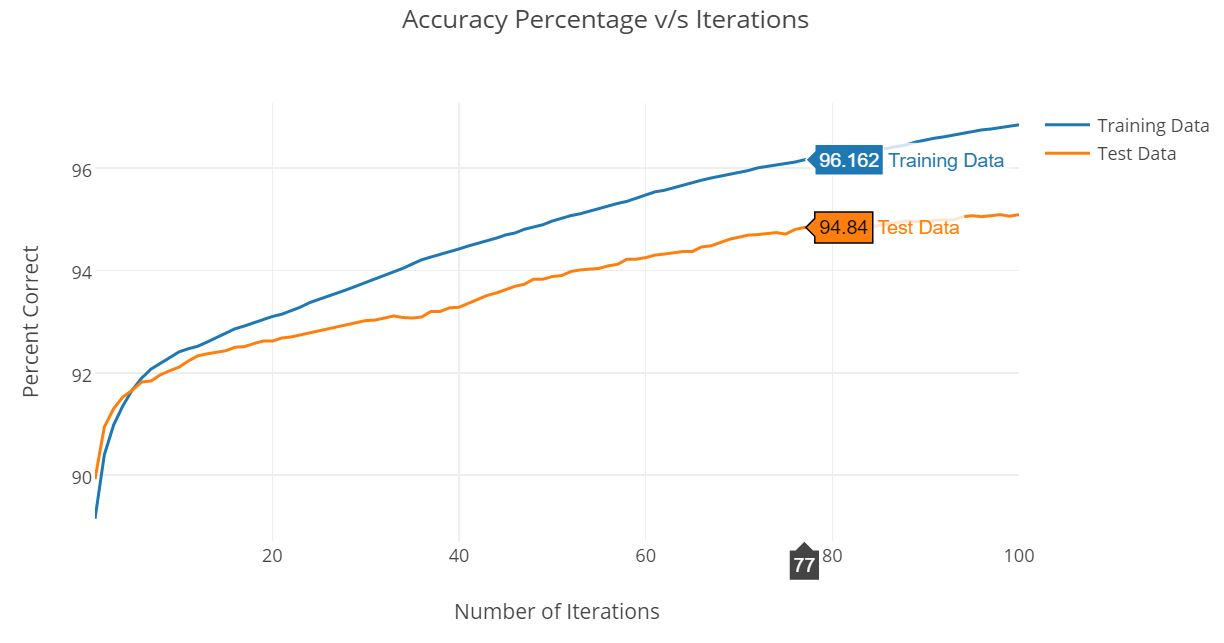
\includegraphics[width=117mm]{graphs/Q4a_point1_50.JPG}
  \caption{Train and test accuracy for mini-batch size 50}
  \label{fig:4a_1}
\end{figure}

\begin{figure}[h!]
  \centering
  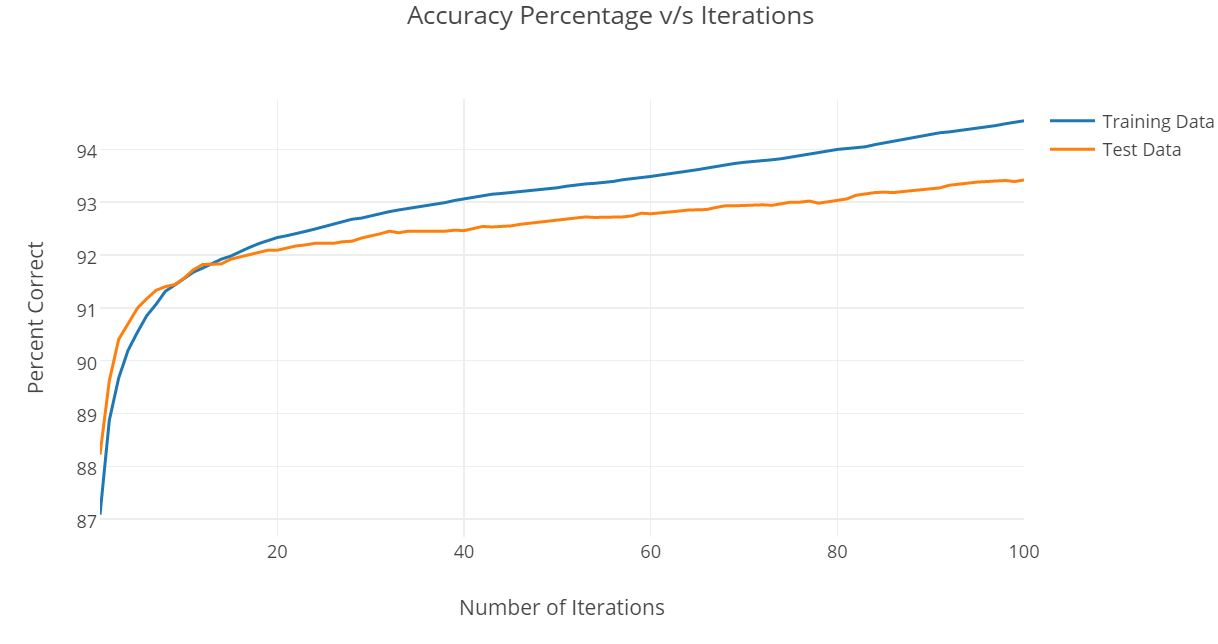
\includegraphics[width=117mm]{graphs/Q4a_point1_128.JPG}
  \caption{Train and test accuracy for mini-batch size 128}
  \label{fig:4a_2}
\end{figure}

\begin{figure}[h!]
  \centering
  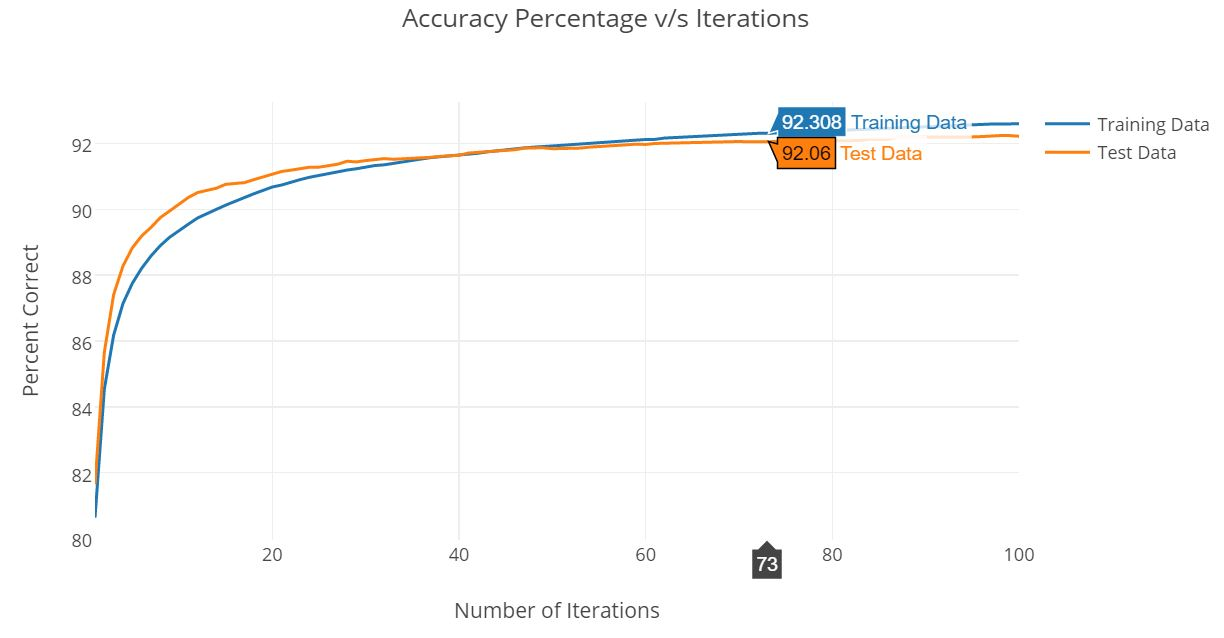
\includegraphics[width=117mm]{graphs/Q4a_point1_500.JPG}
  \caption{Train and test accuracy for mini-batch size 500}
  \label{fig:4a_3}
\end{figure}

2 - Results when using function $1.7159\:tanh(\frac{2x}{3})$ as an activation function for the hidden layer are shown below:

\begin{figure}[h!]
  \centering
  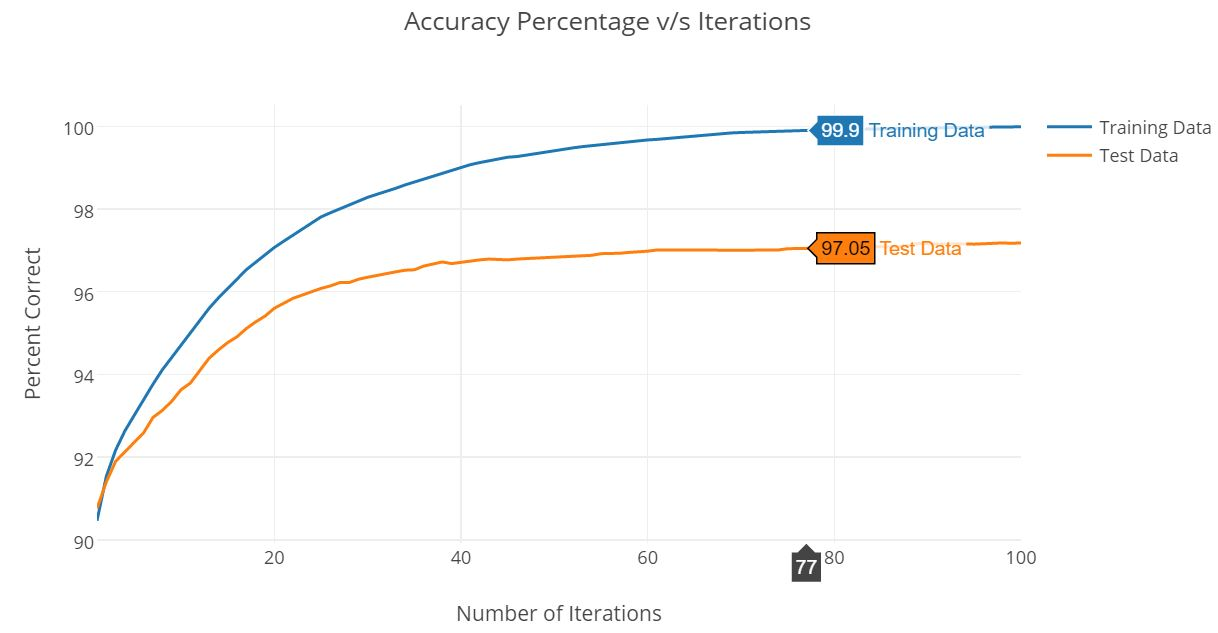
\includegraphics[width=\linewidth]{graphs/Q4c_point1_128_tanh.JPG}
  \caption{Train and test accuracy for tanh activation function with mini-batch size 128}
  \label{fig:4c}
\end{figure}
\pagebreak

3 - Results when weights are sampled from a normal distribution with $\mu=0$ and $\sigma = \sqrt[]{\frac{1}{fan-in}}$

\begin{figure}[h!]
  \centering
  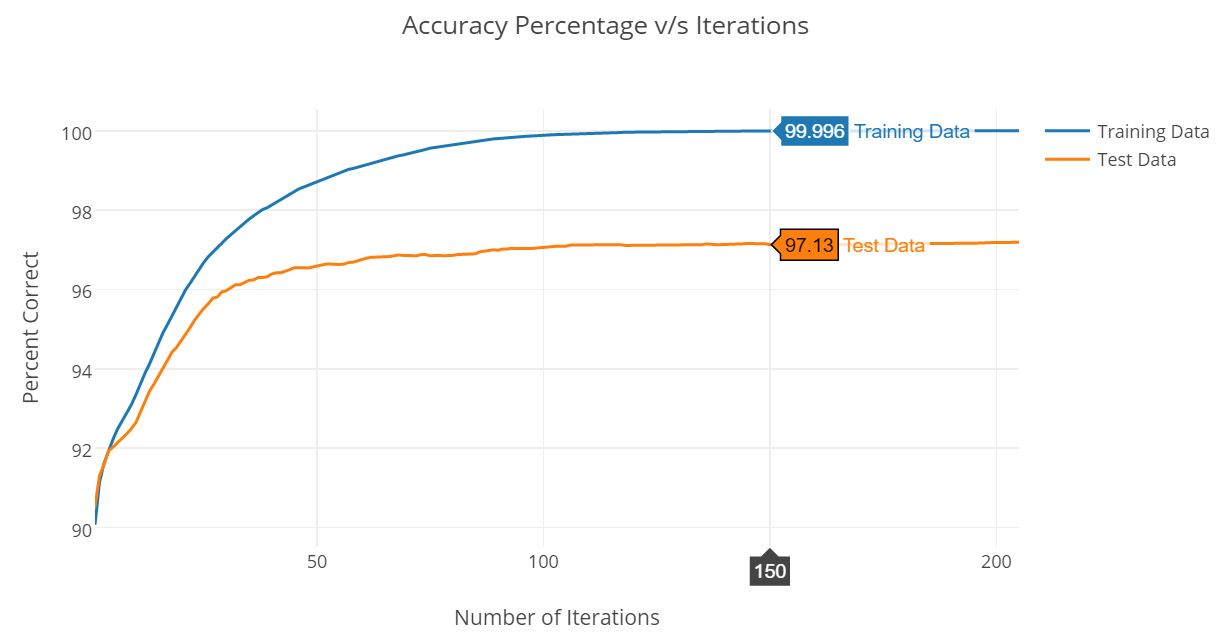
\includegraphics[width=\linewidth]{graphs/Q4d_300HU_point1_500Iter_128.JPG}
  \caption{Train and test accuracy when weights sampled from a normal distribution with $\mu=0$ and $\sigma = \sqrt[]{\frac{1}{fan-in}}$}
  \label{fig:4d}
\end{figure}

4 - Results when momentum term is added in our update rule.
\pagebreak
\begin{figure}[t]
  \centering
  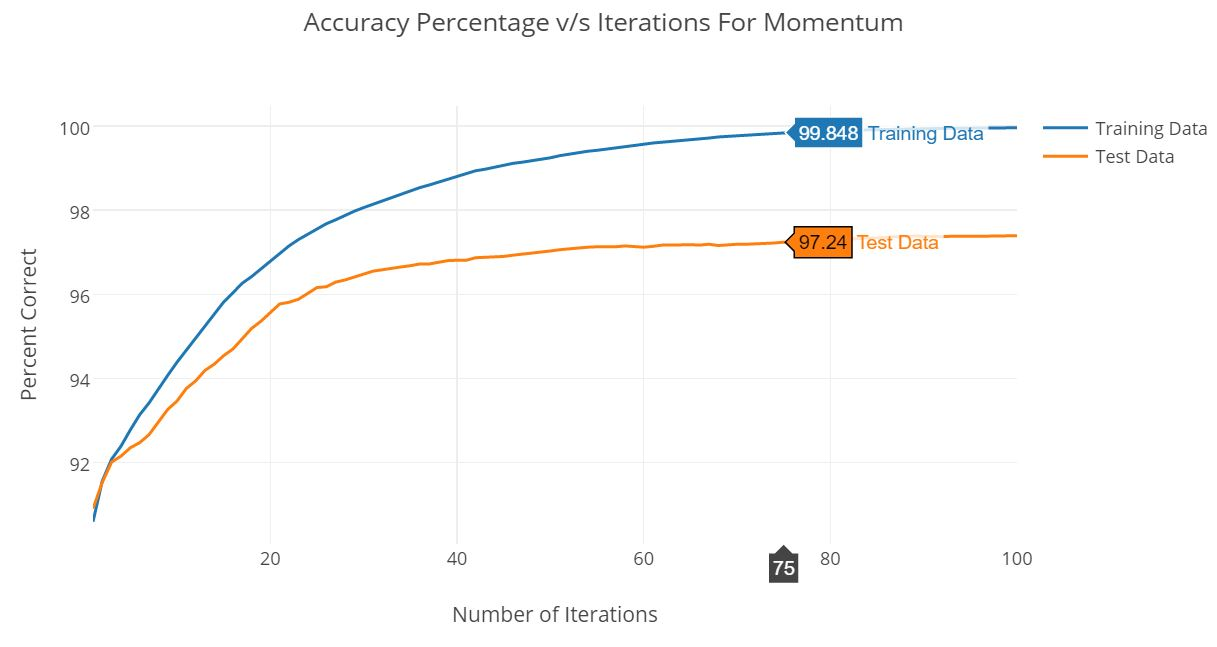
\includegraphics[width=\linewidth]{graphs/Q4e_point9Momentum_point1_128.JPG}
  \caption{Train and test accuracy when we consider momentum with weight 0.9}
  \label{fig:4e}
\end{figure}


\subsection{Discussion}
For the first part, where we introduced the shuffling and mini-batching, the precision when compared with the full batch learning is better by at least 5\% on the test data at 100 epochs (\ref{fig:4a_1} and \ref{fig:3e}). Also, the precision for full batch learning starts from 10\% where as for mini-batches, it starts from 90\%. Mini-batch learning converges faster to a better precision when compared with full-batch learning. This is because mini-batch learning uses noisy gradient to move towards the optimum which results in faster convergence. It might have happened that full-batch learning got stuck at local minima because the precision saturates around 90\% where as for mini-batch learning precision reaches around 95\%. As the number of batches are increased, we see that performance getting a little bit subdued. This is because the gradient become less and less noisy and mini-batch starts having the side effects of full-batch learning. The described behavior is evident from Graphs \ref{fig:4a_1}, \ref{fig:4a_2}, and \ref{fig:4a_3}.   

For the second part, where we chose different sigmoid function for hidden layer, the precision when compared with the case where logistic function was can be clearly seen in graphs \ref{fig:3e}	and \ref{fig:4c}. There's an improvement of about 2\% within 100 epochs. This is because the tanh activation function is symmetric about origin and is more likely to produce output whose mean is close to zero unlike logistic function. Also, we notice that in case of tanh, the convergence is better than that of logistic function.

For the next part, where we initialize the weights using normal distribution with $\mu=0$ and $\sigma = \sqrt[]{\frac{1}{fan-in}}$, we see a slight improvement in the performance when comparing graphs \ref{fig:4c} and \ref{fig:4d}. The difference is not much because prior to this we were initializing the weights using normal distribution with $\mu=0$ and $\sigma = 0.1$. Nevertheless, we can see from the graphs that the convergence speed is slightly improved. This is expected because if the weights are large or small the learning speed would be slow. Our initialization method here ensures that weights are neither too large nor too small.

For the last part, where we will be using a momentum term to update the weights, we see a slight improvement in the convergence rate when comparing graphs \ref{fig:4e} and \ref{fig:4c}. This is expected because the momentum term forces the weights to move into the direction of previous update. If the weights are diverging, momentum would add a positive term to subdue this divergence. Similarly, if weights are converging, momentum would improve the gradient so that the convergence is sped up.

Thus, after applying all the tricks, we can see a lot of improvement in the performance and accuracy from our neural network. This is evident when we compare graphs \ref{fig:3e} and \ref{fig:4e}.

\newpage
\section{Task 5: Experiment with Network Topology}

\subsection{Introduction}

In this section, we would experiment with the network architecture and observe the changes it has on the performance on our dataset.

First, we would change the number of hidden units in our network and analyze the difference. We will try four configuration where the number of hidden units would be 150 (half), 600 (double), 10 (very small) and 1000 (very large) respectively.

Next, we would introduce an additional hidden layer (such that the number of weights parameters are approximately the same as that of single layer) and would analyze the effect it has on the performance on our dataset.

\subsection{Methodology}

For the first part, since we had taken 300 hidden units in the section 4, we would half (150) and double (600) the number of hidden units here to see the effect on performance. All the parameters like learning rate, momentum, batch size, early stopping horizon etc. are same as that of previous part (0.1, 0.9, 128, 5 respectively).

For the second part, we have to introduce one additional hidden layer such that the number of parameters are approximately the same. This means we have to find the solution of following equation:

$$785x + (x+1)*{x}  + (x+1)*10 = 785*300 + 301*10$$
$$796x + x^2 + 10 = 235500 + 3010$$
$$x^2 + 796x - 238500 = 0$$

$$x = \frac{-796 \pm \sqrt[]{796*796 + 4*238500}}{2}$$
$$x  \approx \frac{-796 \pm 1260}{2}$$
$$x  \approx \frac{-796 \pm 1260}{2}$$
$$x  \approx \frac{464}{2} (negative \: x \: not \: possible)$$
$$x  \approx 232$$

Hence, we would consider 232 units (plus 1 bias unit) for each of the hidden layers. All the hyperparameters remain the same as that of previous part. 
We also consider one additional configuration of 300 and 150 hidden units to see the affect of increasing the number of parameters on 2 hidden layer network architecture.

\subsection{Results}

For the part where we have to increase/decrease the number of hidden units in the single layer, the results are shown below:
\pagebreak
\begin{figure}[h!]
  \centering
  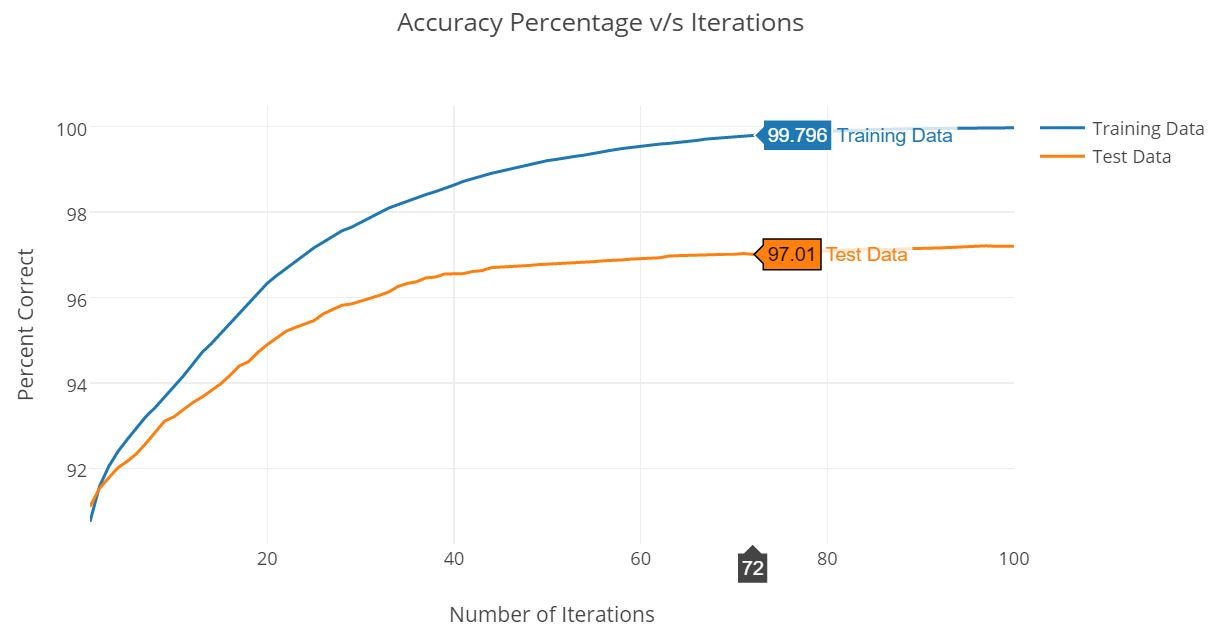
\includegraphics[width=117mm]{graphs/Q5a_600HU.JPG}
  \caption{Train and test accuracy for 1 hidden layer with 600 units}
  \label{fig:5a_1}
\end{figure}

\begin{figure}[h!]
  \centering
  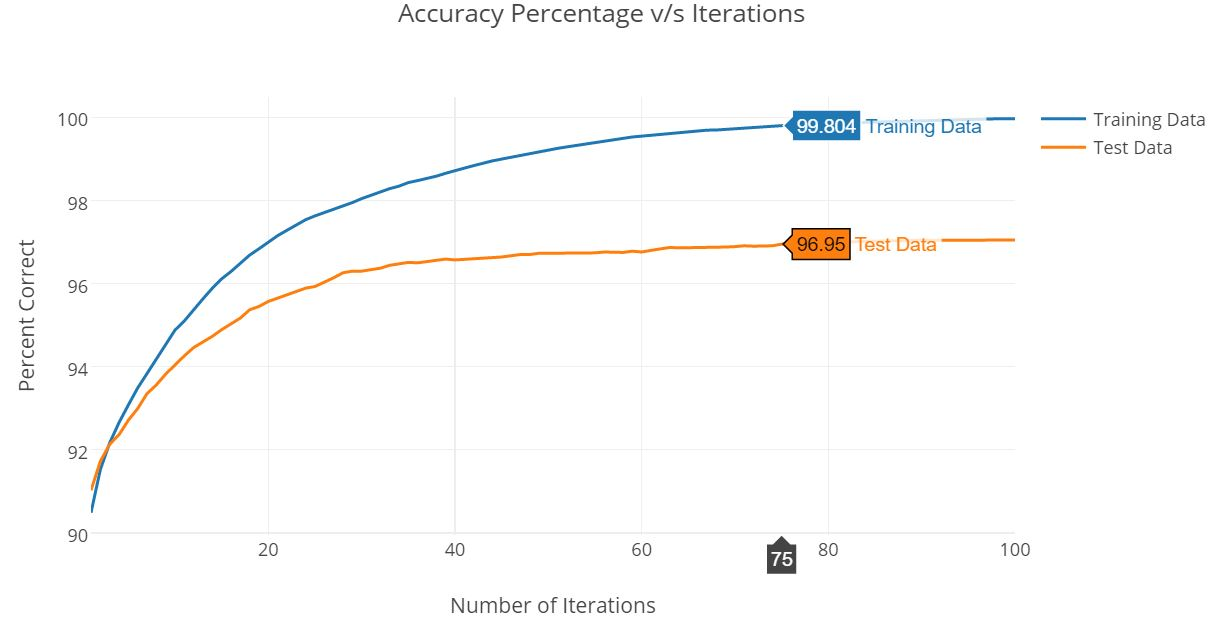
\includegraphics[width=117mm]{graphs/Q5a_150HU.JPG}
  \caption{Train and test accuracy for 1 hidden layer with 150 units}
  \label{fig:5a_2}
\end{figure}

\begin{figure}[h!]
  \centering
  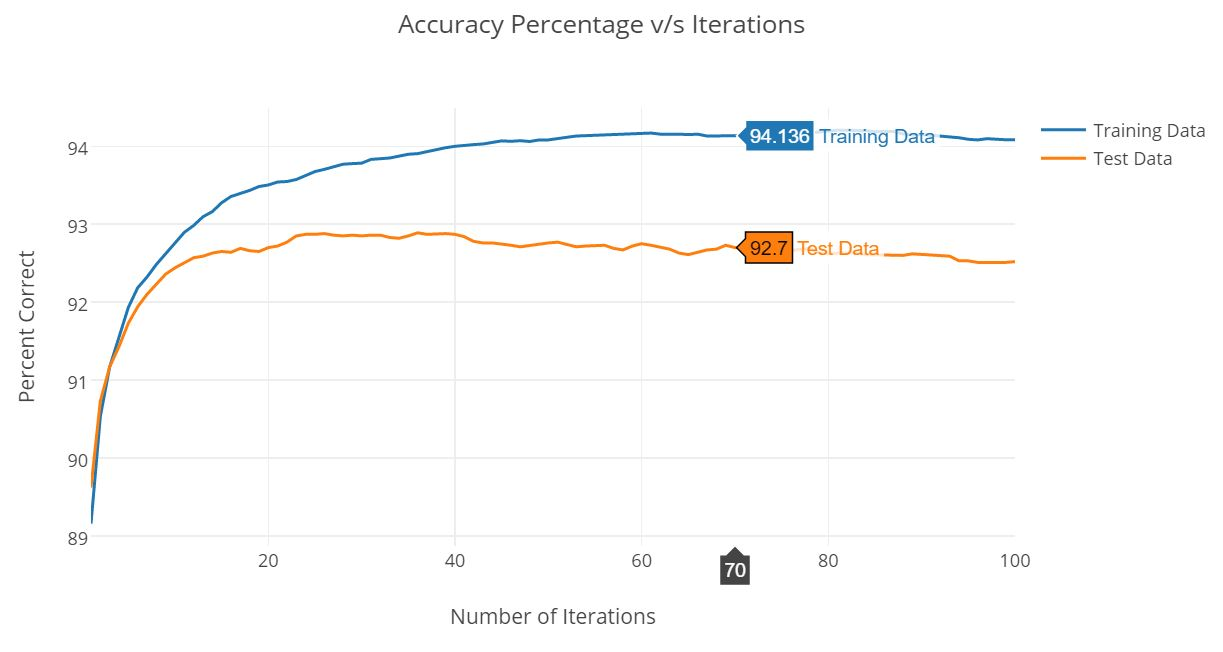
\includegraphics[width=117mm]{graphs/Q5a_10HU.JPG}
  \caption{Train and test accuracy for 1 hidden layer with 10 units}
  \label{fig:5a_3}
\end{figure}

\begin{figure}[h!]
  \centering
  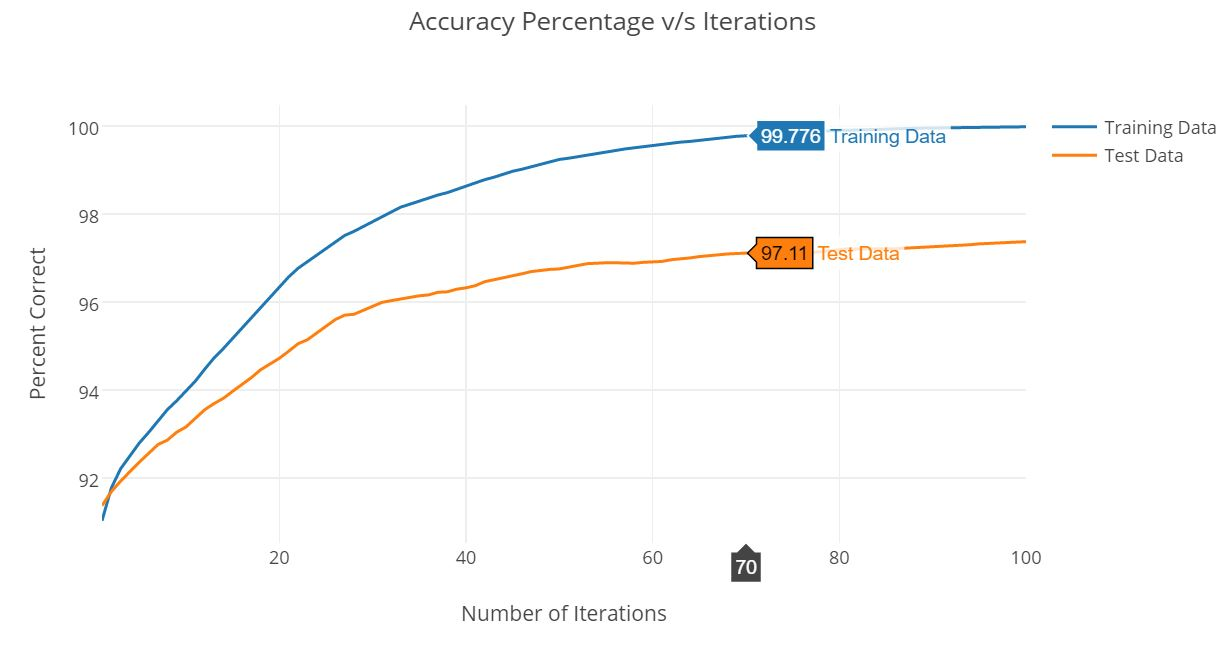
\includegraphics[width=115mm]{graphs/Q5a_1000HU.JPG}
  \caption{Train and test accuracy for 1 hidden layer with 1000 units}
  \label{fig:5a_4}
\end{figure}
\pagebreak
For the part where we have to introduce additional hidden layer, the results are shown below:

\begin{figure}[h!]
  \centering
  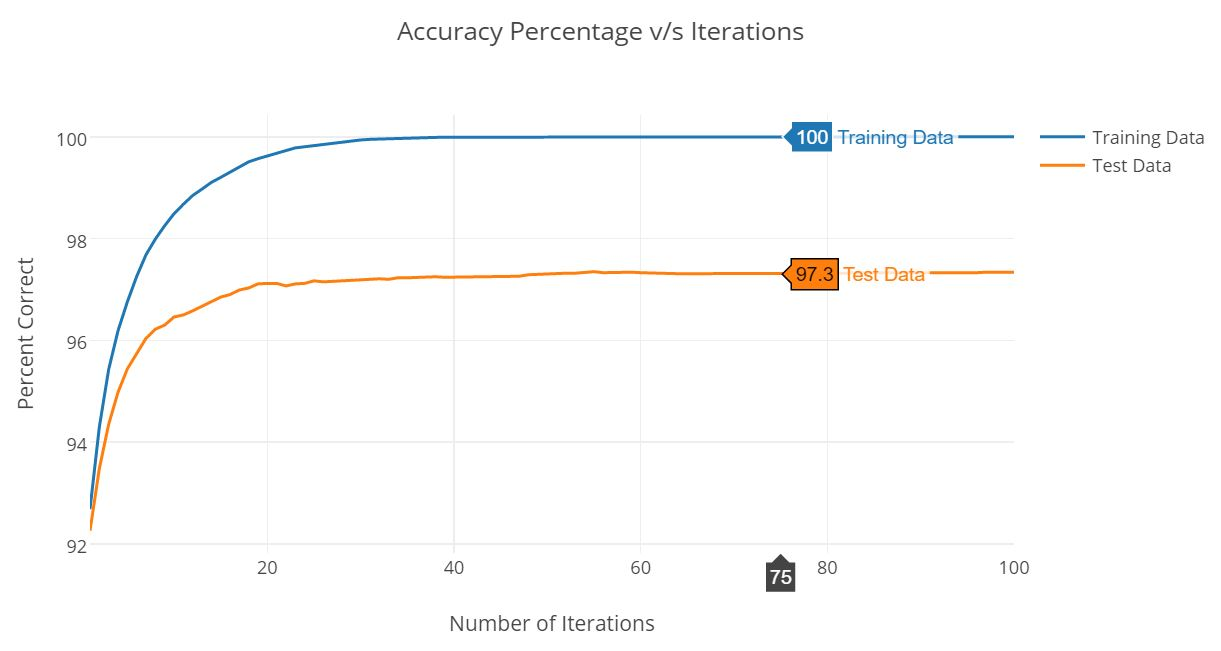
\includegraphics[width=117mm]{graphs/Q5b_232_232HU_point9Mom_point1LR_128BS_500iter.JPG}
  \caption{Train and test accuracy for 2 hidden layers with 232 units each}
  \label{fig:5b_1}
\end{figure}

\begin{figure}[h!]
  \centering
  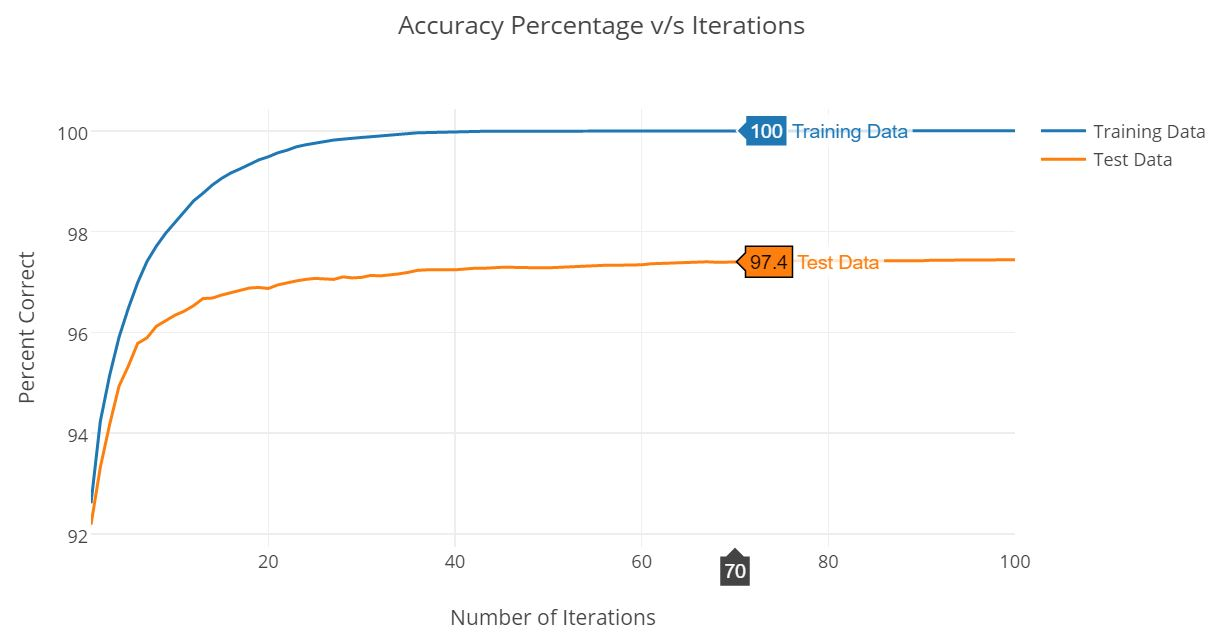
\includegraphics[width=117mm]{graphs/Q5b_300Plus150HU_point9Mom_point1LR_128BS_100iter.JPG}
  \caption{Train and test accuracy for 2 hidden layers with 300 and 150 units repectively}
  \label{fig:5b_2}
\end{figure}

\subsection{Discussion}

Though, the experiments were allowed to run more than 100 epochs with early stopping condition, we are reporting the results of first 100 iteration, where the result has almost converged, to have a better comparative study.

From the Graphs \ref{fig:5a_1}, \ref{fig:5a_2}, \ref{fig:5a_3} and \ref{fig:5a_4}, we infer the following things. When the number of units are very less (10), our network has an overtly less accuracy on both test and train data as compared to the original case (300 units). This is expected as the function learned by our network would be very simplistic and thus the predictions are a bit off. As we increase the number of hidden units, the performance on training as well as test starts to improve. We can see the improvement in performance from graph \ref{fig:5a_2} and \ref{fig:4e} on both test and train data. However, when we increase the hidden units further, we do not see any big improvements in the results. This can be seen from the graph \ref{fig:5a_3} and \ref{fig:5a_4}. The accuracy on test and train is approximately the same. Though, cases with more hidden units takes a bit more time to converge. This could be because more units take more time to get tuned to learn the same function. Also, as we increase the number of units, our method takes more time to perform the same number of epochs as the number of parameters to tune would increase. Hence, our takeaway from this is that after a certain number of units for the hidden layer, we don't see any significant improvement.

For the part where we have to introduce additional layer in our network, we infer the following things from graphs \ref{fig:5b_1} and \ref{fig:5b_2}. For the first graph, the number of parameters are approximately the same as that of the network with 1 layer with 300 units. In the graph, we see slight improvement in accuracy for 2-layered network. This could be because our 2 hidden layered network is capable learning more complex function with arbitrary decision boundaries. One more thing to note is that the weights converge significantly quickly in 2 hidden layered network when compared to 1 hidden layered network. For 2-layered network where the number of parameters are more (300 and 150 units), we see a slight improvement in test data accuracy (train accuracy is already 100\% in both) and convergence is relatively a bit slow. Again, this is because we have more parameters to optimize.

\newpage
\section{Results and Learnings}
The best accuracy on testing data set was achieved to be 97.54\% with two hidden layers, while more than 97\% accuracy was achieved easily using tricks of trades as mentioned by Yann LeCun. Using these tricks improves the learning by a significant amount, saving the developer a lot of time. 

Shuffling and mini-batching improved the performance by almost 5\% and also increased the learning speed. Same goes for the $tanh$ sigmoid function, which seems to be way faster than the traditional logistic sigmoid function. Initializing the weights using normal distribution with $\mu=0$ and $\sigma = \sqrt[]{\frac{1}{fan-in}}$, we see a slight improvement in the performance when comparing graphs \ref{fig:4c} and \ref{fig:4d}. This gives us a good idea as to how to initialize the weights while using neural networks in future. Lastly, we learned the concept of momentum, which plays a great part in correcting the direction of gradient allowing faster and better convergence.

Both of us agree that this programming assignment was definitely an eye-opener for us in the field of neural networks. We had a good time implementing it and experimenting with various values of the learning rate $\eta$. The "tricks of trade" mentioned improved the performance by a significant amount and this is something that we never knew of. We definitely look forward to more of such interactive and practical programming assignments which take more time in implementation and focus on understanding the concepts.

\section{Individual Contributions}
Being roommates, it was extremely convenient and simple for both the authors to coordinate and work in sync, while ensuring equal distribution of work and time spent on the assignment. Whenever one of the authors got stuck at some point, the other was there to help him out and unblock instantly. The authors started out with a plan of having perfectly modularized and re-usable code, so that for question 5, the effort to add another hidden layer would be minimal. The work was taken up as under:

Chetan Gandotra implemented the part which involved reading of MNIST data, normalization of data and forward propagation. Then, Rishabh Misra implemented back-propagation and weight updates. Thereafter, Chetan worked with code for momentum and tanh activation function, and Rishabh worked with the code for 3 (d). The debugging and parameter tuning task was divided equally, with both of the authors testing performance on defined range of parameters. This allowed them to come up with good hyper-parameters fairly  quickly. 

When it came to writing the report, we took up alternate question sub-parts on shared latex file online, ensuring equal work distribution.

\newpage
\section*{References}
\small
[1] LeCun, Yann - Efficient BackProp : http://yann.lecun.com/exdb/publis/pdf/lecun-98b.pdf

\section*{Appendix}
The code consists of three files - LoadMNIST.py, PA2.py and 3d.py

LoadMNIST.py
\begin{lstlisting}
import os, struct
from array import array as pyarray 
from numpy import append, array, int8, uint8, zeros

def load_mnist(dataset="training", digits=None, path=None, asbytes=False, selection=None, return_labels=True, return_indices=False):
    """
    Loads MNIST files into a 3D numpy array.

    You have to download the data separately from [MNIST]_. It is recommended
    to set the environment variable ``MNIST`` to point to the folder where you
    put the data, so that you don't have to select path. On a Linux+bash setup,
    this is done by adding the following to your ``.bashrc``::

        export MNIST=/path/to/mnist

    Parameters
    ----------
    dataset : str 
        Either "training" or "testing", depending on which dataset you want to
        load. 
    digits : list 
        Integer list of digits to load. The entire database is loaded if set to
        ``None``. Default is ``None``.
    path : str 
        Path to your MNIST datafiles. The default is ``None``, which will try
        to take the path from your environment variable ``MNIST``. The data can
        be downloaded from http://yann.lecun.com/exdb/mnist/.
    asbytes : bool
        If True, returns data as ``numpy.uint8`` in [0, 255] as opposed to
        ``numpy.float64`` in [0.0, 1.0].
    selection : slice
        Using a `slice` object, specify what subset of the dataset to load. An
        example is ``slice(0, 20, 2)``, which would load every other digit
        until--but not including--the twentieth.
    return_labels : bool
        Specify whether or not labels should be returned. This is also a speed
        performance if digits are not specified, since then the labels file
        does not need to be read at all.
    return_indicies : bool
        Specify whether or not to return the MNIST indices that were fetched.
        This is valuable only if digits is specified, because in that case it
        can be valuable to know how far
        in the database it reached.

    Returns
    -------
    images : ndarray
        Image data of shape ``(N, rows, cols)``, where ``N`` is the number of images. If neither labels nor inices are returned, then this is returned directly, and not inside a 1-sized tuple.
    labels : ndarray
        Array of size ``N`` describing the labels. Returned only if ``return_labels`` is `True`, which is default.
    indices : ndarray
        The indices in the database that were returned.

    Examples
    --------
    Assuming that you have downloaded the MNIST database and set the
    environment variable ``$MNIST`` point to the folder, this will load all
    images and labels from the training set:

    >>> images, labels = ag.io.load_mnist('training') # doctest: +SKIP

    Load 100 sevens from the testing set:    

    >>> sevens = ag.io.load_mnist('testing', digits=[7], selection=slice(0, 100), return_labels=False) # doctest: +SKIP

    """

    # The files are assumed to have these names and should be found in 'path'
    files = {
        'training': ('train-images.idx3-ubyte', 'train-labels.idx1-ubyte'),
        'testing': ('t10k-images.idx3-ubyte', 't10k-labels.idx1-ubyte'),
    }

    if path is None:
        try:
            path = 'C:\\Users\\Chetan\\Documents\\Python Scripts\\Way1'
            #path = os.environ['MNIST']
        except KeyError:
            raise ValueError("Unspecified path requires environment variable $MNIST to be set")

    try:
        images_fname = os.path.join(path, files[dataset][0])
        labels_fname = os.path.join(path, files[dataset][1])
    except KeyError:
        raise ValueError("Data set must be 'testing' or 'training'")

    # We can skip the labels file only if digits aren't specified and labels aren't asked for
    if return_labels or digits is not None:
        flbl = open(labels_fname, 'rb')
        magic_nr, size = struct.unpack(">II", flbl.read(8))
        labels_raw = pyarray("b", flbl.read())
        flbl.close()

    fimg = open(images_fname, 'rb')
    magic_nr, size, rows, cols = struct.unpack(">IIII", fimg.read(16))
    images_raw = pyarray("B", fimg.read())
    fimg.close()

    if digits:
        indices = [k for k in range(size) if labels_raw[k] in digits]
    else:
        indices = range(size)

    if selection:
        indices = indices[selection] 
    N = len(indices)

    images = zeros((N, rows, cols), dtype=uint8)

    if return_labels:
        labels = zeros((N), dtype=int8)
    for i, index in enumerate(indices):
        images[i] = array(images_raw[ indices[i]*rows*cols : (indices[i]+1)*rows*cols ]).reshape((rows, cols))
        if return_labels:
            labels[i] = labels_raw[indices[i]]

    #if not asbytes:
    #    images = images.astype(float)/255.0

    ret = (images,)
    if return_labels:
        ret += (labels,)
    if return_indices:
        ret += (indices,)
    if len(ret) == 1:
        return ret[0] # Don't return a tuple of one
    else:
        return ret
\end{lstlisting}
PA2.py
\begin{lstlisting}
"""
Variable layer Neural Networks code to Classify Hand-written digits
in MNIST Dataset
"""
import numpy
import math
from LoadMNIST import load_mnist
from sklearn.utils import shuffle
import plotly.plotly as py1
import plotly.graph_objs as go
#import bigfloat

#----------------------------------------Utility functions--------------------------------------#

def get_data(N=60000, N_test=10000, validationReqd = True):
    # Load MNIST data using libraries available
    training_data, training_labels = load_mnist('training')    
    test_data, test_labels = load_mnist('testing')
    
    # Training_data is N x 784 matrix
    training_data = flatten(N, 784, training_data) 
    training_labels = training_labels[:N]
    test_data = flatten(N_test, 784, test_data)
    test_labels = test_labels[:N_test]

    # Adding column of 1s for bias
    training_data = addOnesColAtStart(training_data)
    test_data = addOnesColAtStart(test_data)
    
    if (validationReqd):
        # Last 10% of training data size will be considered as the validation set
        N_validation = int (N / 6.0)
        validation_data = training_data[N-N_validation:N]
        validation_labels = training_labels[N-N_validation:N]
        N=N-N_validation
    else:
        validation_data = []
        validation_labels = []
    
    # Update training data to remove validation data
    training_data = training_data[:N]
    training_labels = training_labels[:N]    

    # Normalization of Data
    training_data = training_data/255.0
    test_data = test_data/255.0
    validation_data = validation_data/255.0
    training_data = training_data - numpy.mean(training_data, axis=0)[numpy.newaxis, :]
    test_data = test_data - numpy.mean(test_data, axis=0)[numpy.newaxis,: ]
    validation_data = validation_data - numpy.mean(validation_data, axis=0)[numpy.newaxis,:]
    
    return training_data, training_labels, test_data, test_labels, validation_data, validation_labels
    
# Convert from tuple form to Matrix form
def flatten(rows, cols, twoDArr):
    flattened_arr = numpy.zeros(shape=(rows, cols))
    for row in range(0, rows):
        i=0
        for element in twoDArr[row]:
            for el1 in element:
                flattened_arr[row][i] = el1
                i = i+1
    return flattened_arr

def addOnesColAtStart(matrix):
    Ones = numpy.ones(len(matrix))
    newMatrix = numpy.c_[Ones, matrix]
    return newMatrix
    
# Single method for calculating sigmoid (logisitic) activation 
# and its derivative
def f_sigmoid(X, derivativeReqd=False):
    if not derivativeReqd:
        return 1.0 / (1 + numpy.exp(-X))
        #return 1.0 / (1 + bigfloat.exp(-X, bigfloat.precision(100)))
    return numpy.multiply(f_sigmoid(X), (1 - f_sigmoid(X)))
 
# Method to calculate the softmax activation
def f_softmax(X):
    Z = numpy.sum(numpy.exp(X), axis=1)
    Z = Z.reshape(Z.shape[0], 1)
    return numpy.exp(X) / Z

# Single method for tanh sigmoid and its derivative
def f_tanh(x, a=0, derivativeReqd = False):
    mul_factor = 1.7159
    div_factor = 2.0/3.0
    tanh_term = numpy.tanh(div_factor*x)
    if not derivativeReqd:
        return (mul_factor * tanh_term + a*x)
    return (div_factor * mul_factor * (1 - (tanh_term*tanh_term))) + a

# Method to return batches from data and labels after shuffling        
def get_batches(X, Y, batch_size):
    N = X.shape[0]
    batch_X = []
    batch_Y = []
    count = 0
    X, Y = shuffle(X, Y, random_state=0)
    while count + batch_size <= N:
        batch_X.append(X[count:count+batch_size, :])
        one_hot = get_one_hot_representation(Y[count:count+batch_size], 10)
        batch_Y.append(one_hot)
        count += batch_size
    return batch_X, batch_Y

# Convert numberical y value (0-9) to a one-hot representation    
def get_one_hot_representation(Y, C=10):
    one_hot = numpy.zeros((Y.shape[0], C))
    for i in range(Y.shape[0]):
        one_hot[i, Y[i]] = 1.0
    return one_hot

# Layer specific forward propogation
def forward_prop(W, Z_prev, layer_no, num_layers, 
                 batch_size, layer_config, activation=f_tanh):
    #Fprime = numpy.zeros((layer_config[layer_no], batch_size))   
    Z = activation(numpy.dot(Z_prev, W))
    if layer_no == num_layers - 1:
        return Z, []
    else:
        # Hidden layers need to have their Fprime values computed
        Fprime = activation(Z, derivativeReqd=True).T
        # Add bias terms for the hidden layers
        Z = numpy.append(numpy.ones((Z.shape[0], 1)), Z, axis=1)
        return Z, Fprime

# Forward propagation begins
def forward_prop_for_all_layers(W, Z, train_data, num_layers,  
                                batch_size, layer_config):
    Z[0] = train_data
    Fprime = []
    for i in range(1, num_layers-1):
        Z[i], Fprime1 = forward_prop(W[i-1], Z[i-1], i, num_layers, 
                                        batch_size, layer_config)
        Fprime.append(Fprime1)
    # Separate call to send f_softmax as the activation function parameter
    Z[-1], Fprime1 = forward_prop(W[-1], Z[-2], num_layers-1, 
                            num_layers, batch_size, layer_config, f_softmax)
    return Z, Fprime

# Backpropagation step
def backprop(y, t, num_layers, Fprime, delta, W):
    delta[-1] = (t - y).T
    for i in range(num_layers-2, 0, -1):
        # Remove the bias column before operating on W
        W1 = W[i][1:, :]
        temp = numpy.dot(W1, delta[i])
        delta[i-1] = numpy.multiply(temp, Fprime[i-1])
    return delta

# Update the weight vectors
def update_weights(learning_rate, num_layers, Z, delta, W, 
                   momentum, prev_del_w):
    ret_val_W_prev = []
    for i in range(0, num_layers-1):
        W_grad = (learning_rate*(numpy.dot(delta[i], Z[i])).T)
        W_grad /= (len(Z[i]))
        ret_val_W_prev.append(W[i])
        W[i] += W_grad + momentum*(W[i] - prev_del_w[i])
    return W, ret_val_W_prev

# Hard coded forward propagation for 2 layer NN - only for testing 
def hard_code_forward_prop(W, Z, num_layers, 
                           batch_size, layer_config):
    A = []
    A.append(numpy.dot(Z[0], W[0]))
    Z[1] = f_sigmoid(A[0])
    Fprime = []
    Fprime.append(f_sigmoid(Z[1], derivativeReqd=True).T)
    Z[1] = numpy.append(numpy.ones((Z[1].shape[0], 1)), Z[1], axis=1)
    A.append(numpy.dot(Z[1], W[1]))
    Z[2] = f_softmax(A[1])
    return Z, Fprime

# train the model
def fit(X, y, X_test, y_test, X_val, y_val, iterations, learning_rate, 
        num_layers, W, Z, Z_val, Z_test, delta,   
        batch_size, layer_config, batch_size_val, batch_size_test,
        momentum, prev_del_W):
            
    train_data_batches, train_label_batches = get_batches(X, y, 
                                                          batch_size)        
    val_data_batches, val_label_batches = get_batches(X_val, y_val, 
                                                      batch_size_val)
    test_data_batches, test_label_batches = get_batches(X_test, y_test, 
                                                       batch_size_test)
    
    percent_correct_train = []    
    percent_correct_test = []    
    weights_array= []
    val_error_array = []
    test_error = 0.0
    stopping_threshold = 20
    W_opt = W    
    
    for t in range(iterations):
        # Train for particular iteration
        for i in range(len(train_label_batches)):
            batch_data = train_data_batches[i]
            batch_labels = train_label_batches[i]
            # Forward Propagation   
            Z_updated, Fprime = forward_prop_for_all_layers(W, Z,
                                                             batch_data, 
                                                             num_layers, 
                                                             batch_size, 
                                                             layer_config)
            # Back-propagation                                                 
            delta = backprop(Z_updated[-1], batch_labels, num_layers,
                             Fprime, delta, W)
            # Update the weights
            W, prev_del_W = update_weights(learning_rate, num_layers,
                               Z_updated, delta, W, momentum, prev_del_W)
                
        # Check error on training data for this iteration 
        # and add to plot array
        train_error = find_misclassification_error(train_data_batches,
                                                   train_label_batches,
                                                   Z, W)
        percent_correct_train.append(((1-train_error/len(y))*100))
        
        # Check error on validation data for this iteration
        val_error = find_misclassification_error(val_data_batches, 
                                                 val_label_batches,
                                                 Z_val, W)
        print ("Validation error = " + str(val_error/len(y_val)) 
                + " iteration number = " + str(t))

        weights_array.append(W)
        val_error_array.append(val_error)
        W_opt = W

        # Check error on Test Data and add to test plot array
        test_error = find_misclassification_error(test_data_batches, 
                                                  test_label_batches, 
                                                  Z_test, W)
        percent_correct_test.append(((1-test_error/len(y_test))*100))
        
        # Setting threshold of minimum 15 iterations before we abort
        if (early_stop_reqd(t, stopping_threshold, val_error_array)):
            W_opt = weights_array[numpy.argmin(val_error_array)] 
            break
        
    # Check error on Test Data with final weight vector chosen
    test_error = find_misclassification_error(test_data_batches, 
                                              test_label_batches, 
                                              Z_test, W_opt)
    print ("Test error = " + str(test_error/len(y_test)))
    plotly_graphs(percent_correct_train, percent_correct_test)
    
def early_stop_reqd(t, stopping_threshold, val_error_array):
    if (t > stopping_threshold):
        count = 0
        for index in range(t - 1, t-stopping_threshold, -1):
            if (count < stopping_threshold 
            and val_error_array[index] >= val_error_array[index-1]):
                count += 1
            else:
                return False
        if (count >= stopping_threshold - 1):
           return True
    return False
        
# Find the misclassification error given batches of labels and data
def find_misclassification_error(data_batches, label_batches, Z, W):
    error = 0.0
    for i in range(len(label_batches)):
        batch_data = data_batches[i]
        batch_labels = label_batches[i]
        Z_updated, Fprime_test = forward_prop_for_all_layers(W, 
                                                         Z, 
                                                         batch_data,
                                                         num_layers, 
                                                         batch_size_test, 
                                                         layer_config)
        y_pred = numpy.argmax(Z_updated[-1], axis=1)
        error += numpy.sum(1-batch_labels[numpy.arange(len(batch_labels)), 
                                           y_pred])    
    return error
                                           
# Plot Percent correct graphs for testing and training data using Plotly
def plotly_graphs(percent_correct_train, percent_correct_test):
    py1.sign_in('chetang', 'vil7vTAuCSWt2lEZvaH9')
    trace = []
    graph_y = []
    graph_y.append(percent_correct_train)
    graph_y.append(percent_correct_test)
    for i in range(2):
        name = "Training Data"
        if i == 1:
            name = "Test Data"
        y1 = graph_y[i]
        x1 = [j+1 for j in range(len(y1))]
        trace1 = go.Scatter(
            x=x1,
            y=y1,
            name = name,
            connectgaps=True
        )
        trace.append(trace1)
    data = trace
    fig = dict(data=data)
    py1.iplot(fig, filename='5b_232_232HU_Point1_128BS_point9M')
        
#---------------------------------------Main function------------------------------------------------------
        
if __name__ == "__main__":     
    numpy.random.seed(0)
    learning_rate = 0.22
    momentum = 0.0
    N = 60000
    N_test = 10000
    iteration = 2000
    X, y, X_test, y_test, X_validation, y_validation = get_data(N, 
                                                                N_test, 
                                                                True)
    batch_size = 50000
    batch_size_val = 10000
    batch_size_test = 10000
    
    # Layers - 784, 300, 10
    layer_config = [784, 300, 10]
    num_layers = len(layer_config)
    W = []
    Z = []
    Z_test = []
    Z_val = []
    delta = []
    prev_del_W = []
        
    for i in range(num_layers): 
        # common for all layers except input layer
        if i != 0:
            Z.append(numpy.zeros((batch_size, layer_config[i])))
            Z_test.append(numpy.zeros((batch_size_test, layer_config[i])))
            Z_val.append(numpy.zeros((batch_size_val, layer_config[i])))
            delta.append(numpy.zeros((batch_size, layer_config[i])))
        else:
            Z.append(numpy.zeros((batch_size, layer_config[i]+1)))
            Z_test.append(numpy.zeros((batch_size_test, layer_config[i]+1)))
            Z_val.append(numpy.zeros((batch_size_val, layer_config[i]+1)))
        # For all layers except output
        if i != num_layers - 1:
            W.append(numpy.random.normal(size=[layer_config[i]+1, 
                                               layer_config[i+1]], 
                                               loc = 0.0, 
                                               #scale = 0.1))
                                               scale = 1.0/math.sqrt(layer_config[i])))
            prev_del_W.append(numpy.zeros((layer_config[i]+1, 
                                               layer_config[i+1])))
                                               
    fit(X, y, X_test, y_test, X_validation, y_validation, iteration, 
        learning_rate, num_layers, W, 
        Z, Z_val, Z_test, delta,  
        batch_size, layer_config,
        batch_size_val, batch_size_test, momentum, prev_del_W)
\end{lstlisting}
3d.py
\begin{lstlisting}

import numpy
from LoadMNIST import load_mnist
from sklearn.utils import shuffle
import plotly.plotly as py1
import plotly.graph_objs as go
import copy
#import bigfloat

#----------------------------------------Utility functions--------------------------------------#

def get_data(N=60000, N_test=10000, validationReqd = True):
    # Load MNIST data using libraries available
    training_data, training_labels = load_mnist('training')    
    test_data, test_labels = load_mnist('testing')
    
    # Training_data is N x 784 matrix
    training_data = flattenAndNormalize(N, 784, training_data) 
    training_labels = training_labels[:N]
    test_data = flattenAndNormalize(N_test, 784, test_data)
    test_labels = test_labels[:N_test]

    # Adding column of 1s for bias
    training_data = addOnesColAtStart(training_data)
    test_data = addOnesColAtStart(test_data)
    
    if (validationReqd):
        # Last 10% of training data size will be considered as the validation set
        N_validation = int (N / 6.0)
        validation_data = training_data[N-N_validation:N]
        validation_labels = training_labels[N-N_validation:N]
        N=N-N_validation
    else:
        validation_data = []
        validation_labels = []
    #update training data to remove validation data
    training_data = training_data[:N]
    training_labels = training_labels[:N]    

    return training_data, training_labels, test_data, test_labels, validation_data, validation_labels
    
def flattenAndNormalize(rows, cols, twoDArr):
    flattened_arr = numpy.zeros(shape=(rows, cols))
    for row in range(0, rows):
        i=0
        for element in twoDArr[row]:
            for el1 in element:
                flattened_arr[row][i] = el1
                i = i+1
    return flattened_arr

def addOnesColAtStart(matrix):
    Ones = numpy.ones(len(matrix))
    newMatrix = numpy.c_[Ones, matrix]
    return newMatrix
    
# Single method for calculating sigmoid (logisitic) activation 
# and its derivative
def f_sigmoid(X, derivativeReqd=False):
    if not derivativeReqd:
        return 1.0 / (1 + numpy.exp(-X))
        #return 1.0 / (1 + bigfloat.exp(-X, bigfloat.precision(100)))
    return numpy.multiply(f_sigmoid(X), (1 - f_sigmoid(X)))

# Method to calculate the softmax activation
def f_softmax(X):
    Z = numpy.sum(numpy.exp(X), axis=1)
    Z = Z.reshape(Z.shape[0], 1)
    return numpy.exp(X) / Z

# Single method for tanh sigmoid and its derivative
def f_tanh(x, a=0, derivativeReqd = False):
    mul_factor = 1.7159
    div_factor = 2.0/3.0
    tanh_term = numpy.tanh(div_factor*x)
    if not derivativeReqd:
        return (mul_factor * tanh_term + a*x)
    return (div_factor * mul_factor * (1 - (tanh_term*tanh_term))) + a

# Method to return batches from data and labels after shuffling        
def get_batches(X, Y, batch_size):
    N = len(X)#X.shape[0]
    batch_X = []
    batch_Y = []
    count = 0
    X, Y = shuffle(X, Y, random_state=0)
    while count + batch_size <= N:
        batch_X.append(X[count:count+batch_size, :])
        one_hot = get_one_hot_representation(Y[count:count+batch_size], 10)
        batch_Y.append(one_hot)
        count += batch_size
    return batch_X, batch_Y

# Convert numberical y value (0-9) to a one-hot representation    
def get_one_hot_representation(Y, C=10):
    one_hot = numpy.zeros((Y.shape[0], C))
    for i in range(Y.shape[0]):
        one_hot[i, Y[i]] = 1.0
    return one_hot

# Layer specific forward propogation
def forward_prop(W, Z_prev, layer_no, num_layers, 
                 batch_size, layer_config, activation=f_sigmoid):
    #Fprime = numpy.zeros((layer_config[layer_no], batch_size))   
    Z = activation(numpy.dot(Z_prev, W))
    if layer_no == num_layers - 1:
        return Z, []
    else:
        # Hidden layers need to have their Fprime values computed
        Fprime = activation(Z, derivativeReqd=True).T
        # Add bias terms for the hidden layers
        Z = numpy.append(numpy.ones((Z.shape[0], 1)), Z, axis=1)
        return Z, Fprime

# Forward propagation begins
def forward_prop_for_all_layers(W, Z, train_data, num_layers,  
                                batch_size, layer_config):
    Z[0] = train_data
    Fprime = []
    for i in range(1, num_layers-1):
        Z[i], Fprime1 = forward_prop(W[i-1], Z[i-1], i, num_layers, 
                                        batch_size, layer_config)
        Fprime.append(Fprime1)
    # Separate call to send f_softmax as the activation function parameter
    Z[-1], Fprime1 = forward_prop(W[-1], Z[-2], num_layers-1, 
                            num_layers, batch_size, layer_config, f_softmax)
    return Z, Fprime

# Backpropagation step
def backprop(y, t, num_layers, Fprime, delta, W):
    delta[-1] = (t - y).T
    for i in range(num_layers-2, 0, -1):
        # Remove the bias column before operating on W
        W1 = W[i][1:, :]
        temp = numpy.dot(W1, delta[i])
        delta[i-1] = numpy.multiply(temp, Fprime[i-1])
    return delta

# Update the weight vectors
def update_weights(learning_rate, num_layers, Z, delta, W, 
                   momentum, prev_del_w, size):
    ret_val_W_prev = []
    gradient_bp = []
    for i in range(0, num_layers-1):
        W_grad = (learning_rate*(numpy.dot(delta[i], Z[i])).T + momentum*prev_del_w[i])/float(size);
        gradient_bp.append(W_grad)
        W[i] += W_grad
        ret_val_W_prev.append(-1*W_grad)
    return W, ret_val_W_prev, gradient_bp

# Update the weight vectors
def update_weights_analytical_gradient(learning_rate, num_layers, Z, delta, W, t, activation_hidden = f_sigmoid, activation_output = f_softmax):
    e = 0.01
    gradient = []
    W_save = copy.deepcopy(W)
    for x in range(0, num_layers-1):
        gradient.append(numpy.zeros((W[x].shape[0], W[x].shape[1])))
        for i in range(0,W[x].shape[0]):
            for j in range(0,W[x].shape[1]):
                W_pos = copy.deepcopy(W_save)
                W_neg = copy.deepcopy(W_save)
                
                W_pos[x][i][j] = W_save[x][i][j] + e
                W_neg[x][i][j] = W_save[x][i][j] - e
                #print(W_save[x][i][j] - W_pos[x][i][j])
                Z_pos = copy.deepcopy(Z)
                Z_neg = copy.deepcopy(Z)
                for k in range(1,num_layers-1):
                    Z_pos[k] = activation_hidden(numpy.dot(Z_pos[k-1], W_pos[k-1]))
                    Z_neg[k] = activation_hidden(numpy.dot(Z_neg[k-1], W_neg[k-1]))
                    Z_pos[k] = numpy.append(numpy.ones((Z_pos[k].shape[0], 1)), Z_pos[k], axis=1)
                    Z_neg[k] = numpy.append(numpy.ones((Z_neg[k].shape[0], 1)), Z_neg[k], axis=1)                    
        
                Z_pos[-1] = activation_output(numpy.dot(Z_pos[-2], W_pos[-1]))
                Z_neg[-1] = activation_output(numpy.dot(Z_neg[-2], W_neg[-1]))

                gradient[x][i][j] = ( learning_rate * (numpy.dot(t, numpy.log(Z_pos[-1].T)) - numpy.dot(t, numpy.log(Z_neg[-1].T))) / 2.0*e)                   
                
    return gradient
    
# Hard coded forward propagation for 2 layer NN - only for testing 
def hard_code_forward_prop(W, Z, num_layers, 
                           batch_size, layer_config):
    A = []
    A.append(numpy.dot(Z[0], W[0]))
    Z[1] = f_sigmoid(A[0])
    Fprime = []
    Fprime.append(f_sigmoid(Z[1], derivativeReqd=True).T)
    Z[1] = numpy.append(numpy.ones((Z[1].shape[0], 1)), Z[1], axis=1)
    A.append(numpy.dot(Z[1], W[1]))
    Z[2] = f_softmax(A[1])
    return Z, Fprime

# train the model
def fit(X, y, X_test, y_test, X_val, y_val, iterations, learning_rate, 
        num_layers, W, Z, Z_val, Z_test, delta,   
        batch_size, layer_config, batch_size_val, batch_size_test,
        momentum, prev_del_W):
            
    train_data_batches, train_label_batches = get_batches(X, y, 
                                                          batch_size)        
    val_data_batches, val_label_batches = get_batches(X_val, y_val, 
                                                      batch_size_val)
    test_data_batches, test_label_batches = get_batches(X_test, y_test, 
                                                       batch_size_test)
    
    test_error = 0.0
    
    for t in range(iterations):
        # Train for particular iteration
        for i in range(len(train_label_batches)):
            batch_data = train_data_batches[i]
            batch_labels = train_label_batches[i]
            # Forward Propagation   
                     
            Z_updated, Fprime = forward_prop_for_all_layers(W, Z,
                                                             batch_data, 
                                                             num_layers, 
                                                             batch_size, 
                                                             layer_config)
            # Back-propagation                                                 
            delta = backprop(Z_updated[-1], batch_labels, num_layers,
                             Fprime, delta, W)
            # Update the weights
            W_true, prev_del_W, gradient_bp = update_weights(learning_rate, num_layers,
                               Z_updated, delta, W, momentum, prev_del_W, len(batch_labels))
            
            # Update the weights
            gradient_ana = update_weights_analytical_gradient(learning_rate, num_layers,
                               Z_updated, delta, W, batch_labels)
            
            gradient_bp = [gradient_bp[i] - gradient_ana[i] for i in range(0,len(gradient_bp))]
            print(gradient_bp)            
            
            diff_grad_ij = numpy.fabs(gradient_bp[0] - gradient_ana[0])
            diff_grad_jk = numpy.fabs(gradient_bp[1] - gradient_ana[1])

            max_diff_ij = numpy.amax(diff_grad_ij)
            max_diff_jk = numpy.amax(diff_grad_jk)    
            mean_diff_ij = numpy.mean(diff_grad_ij)
            mean_diff_jk = numpy.mean(diff_grad_jk)
            print("max_diff_ij: " + str(max_diff_ij))
            print("max_diff_jk: " + str(max_diff_jk))
            
            print("mean_diff_ij: " + str(mean_diff_ij))
            print("mean_diff_jk: " + str(mean_diff_jk))

            numpy.savetxt("Gradient_diff.csv", gradient_bp[0], delimiter=",")
            numpy.savetxt("Gradient_diff2.csv", gradient_bp[1], delimiter=",")
                
    print ("Test error = " + str(test_error/len(y_test)))
    
def plotly_graphs(percent_correct_train, percent_correct_test):
    py1.sign_in('chetang', 'vil7vTAuCSWt2lEZvaH9')
    trace = []
    graph_y = []
    graph_y.append(percent_correct_train)
    graph_y.append(percent_correct_test)
    for i in range(2):
        name = "Training Data"
        if i == 1:
            name = "Test Data"
        y1 = graph_y[i]
        x1 = [j+1 for j in range(len(y1))]
        trace1 = go.Scatter(
            x=x1,
            y=y1,
            name = name,
            connectgaps=True
        )
        trace.append(trace1)
    data = trace
    fig = dict(data=data)
    py1.iplot(fig, filename='percentCorrect-connectgaps_1')
        
#---------------------------------------Main function------------------------------------------------------
        
if __name__ == "__main__":     
    numpy.random.seed(0)
    learning_rate = 0.001
    momentum = 0.0
    N = 1
    N_test = 1
    iteration = 1
    X, y, X_test, y_test, X_validation, y_validation = get_data(N, 
                                                                N_test, 
                                                                False)
    X = X/255.0
    #X_test = X_test/255.0
    #X_validation = X_validation/255.0
    #X = X - numpy.mean(X, axis=0)[numpy.newaxis, :]
    for r in range(0,X.shape[0]):
        X[r] = X[r] - sum(X[r])/X.shape[1]
    #X_test = X_test - numpy.mean(X_test, axis=0)[numpy.newaxis,: ]
    #X_validation = X_validation - numpy.mean(X_validation, axis=0)[numpy.newaxis,:]
    
    batch_size = 1
    batch_size_val = 1
    batch_size_test = 1
    
    # Layers - 784, 100, 10
    layer_config = [784, 300, 10]
    num_layers = len(layer_config)
    W = []
    Z = []
    Z_test = []
    Z_val = []
    delta = []
    prev_del_W = []
        
    for i in range(num_layers): 
        # common for all layers except input layer
        if i != 0:
            Z.append(numpy.zeros((batch_size, layer_config[i])))
            Z_test.append(numpy.zeros((batch_size_test, layer_config[i])))
            Z_val.append(numpy.zeros((batch_size_val, layer_config[i])))
            delta.append(numpy.zeros((batch_size, layer_config[i])))
        else:
            Z.append(numpy.zeros((batch_size, layer_config[i]+1)))
            Z_test.append(numpy.zeros((batch_size_test, layer_config[i]+1)))
            Z_val.append(numpy.zeros((batch_size_val, layer_config[i]+1)))
        # For all layers except output
        if i != num_layers - 1:
            W.append(numpy.random.normal(size=[layer_config[i]+1, 
                                               layer_config[i+1]], 
                                               loc = 0.0, 
                                               scale=0.001))
            prev_del_W.append(numpy.zeros((layer_config[i]+1, 
                                               layer_config[i+1])))
                                               
    fit(X, y, X_test, y_test, X_validation, y_validation, iteration, 
        learning_rate, num_layers, W, 
        Z, Z_val, Z_test, delta,  
        batch_size, layer_config,
        batch_size_val, batch_size_test, momentum, prev_del_W)
\end{lstlisting}
\end{document}
